\section{Proceso de Seguimiento y Control} 

  En esta sección se describen los procesos de seguimiento y control del proyecto, que incluyen la supervisión del progreso, la gestión de cambios, la evaluación del desempeño y la implementación de acciones correctivas cuando sea necesario. Estos procesos son esenciales para garantizar que el proyecto se mantenga en línea con los objetivos establecidos y se complete dentro del alcance, tiempo y presupuesto definidos.

  \subsection{Gestión de la Integración}

    La gestión de la integración del proyecto implica coordinar todos los aspectos del proyecto para asegurar que se trabajen de manera coherente y eficiente. Esto incluye la elaboración del plan de gestión del proyecto, la dirección y gestión del trabajo del proyecto, el monitoreo y control del trabajo del proyecto, y la realización del control integrado de cambios.

    \textbf{Objetivo:} Asegurar que todos los elementos del proyecto estén alineados y se gestionen de manera integrada para lograr los objetivos del proyecto.

    A continuación se presenta 

% Inserta todas las páginas del PDF
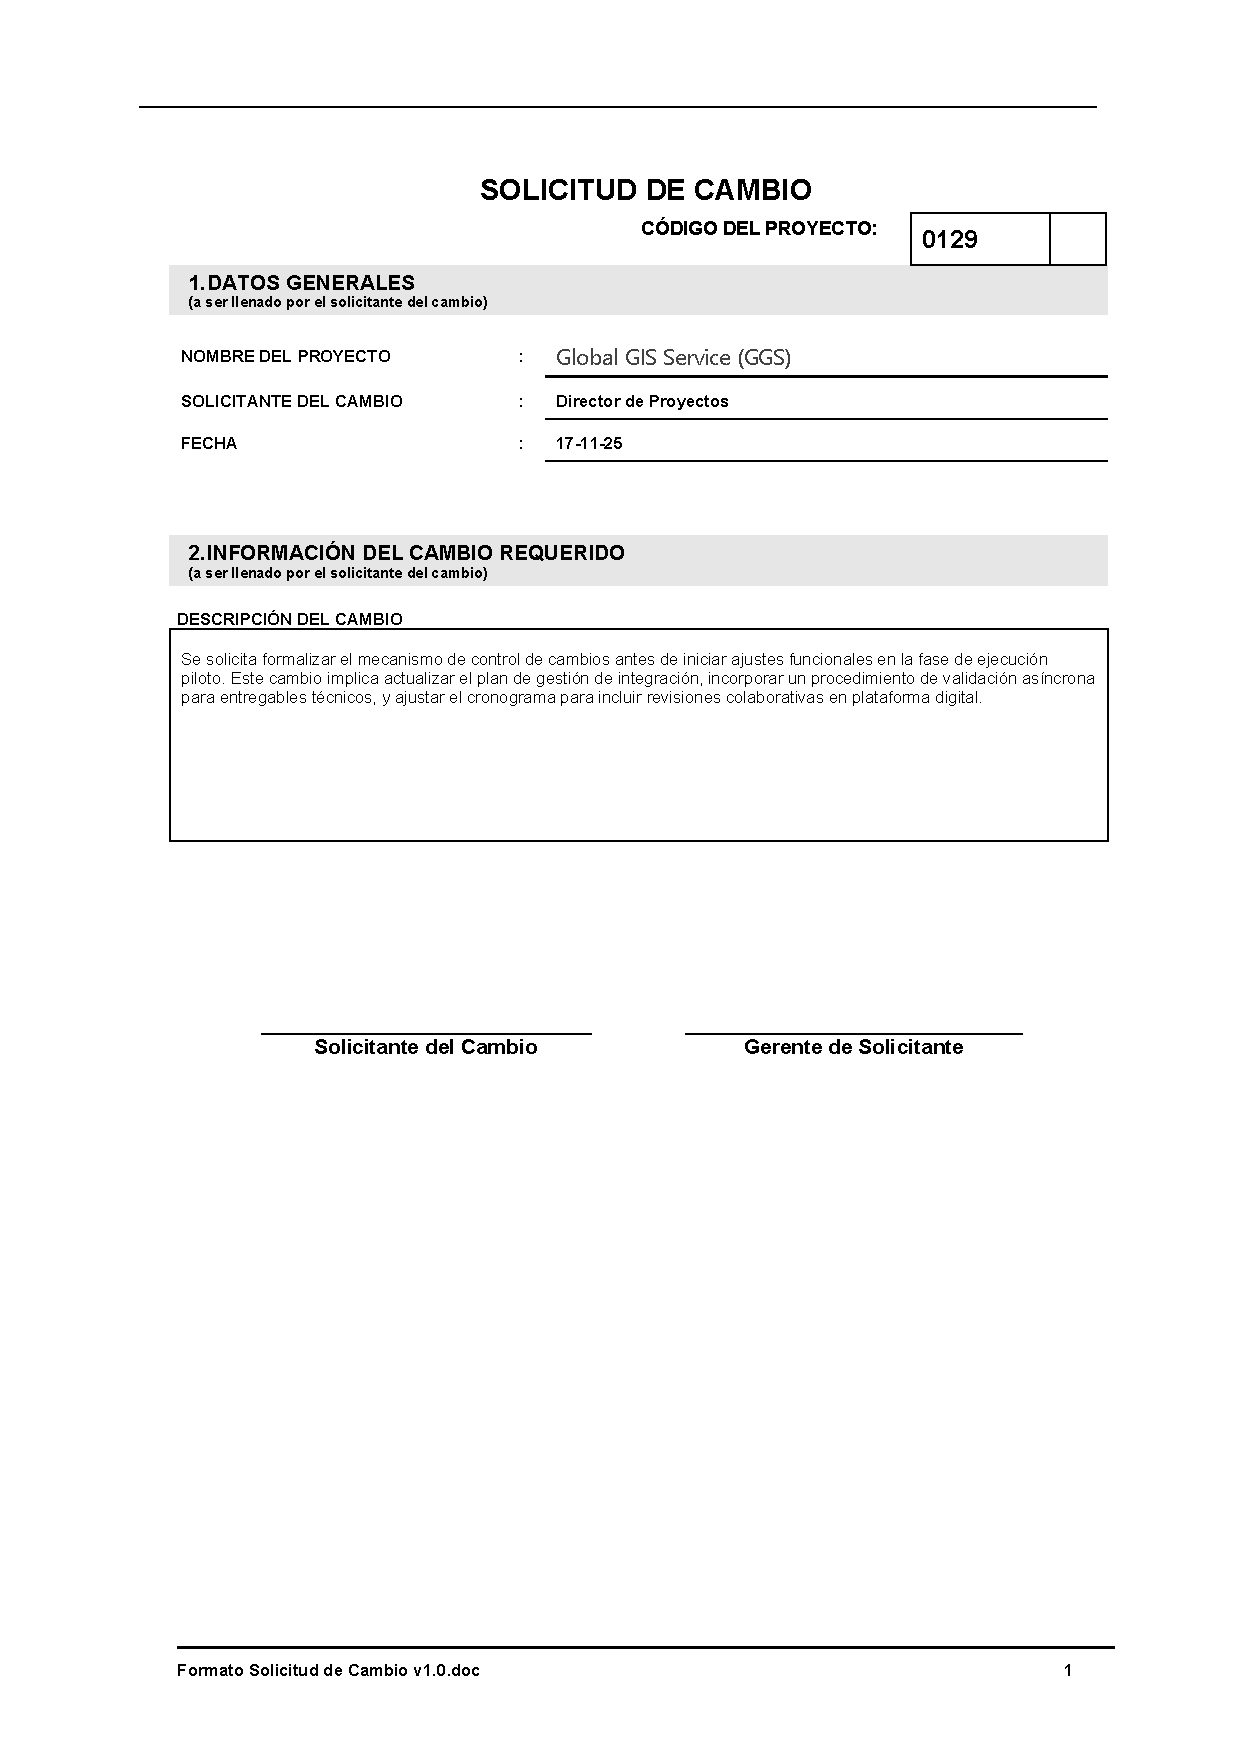
\includepdf[pages=-]{qq.pdf}

\subsection{Gestión del Alcance}

    La gestión del alcance del proyecto implica definir y controlar qué está incluido y qué no está incluido en el proyecto. Esto incluye la recopilación de requisitos, la definición del alcance, la creación de la estructura de desglose del trabajo (EDT), la verificación del alcance y el control del alcance.

    \textbf{Objetivo:} Asegurar que el proyecto incluya todo el trabajo necesario para completar el proyecto con éxito, evitando el trabajo adicional no planificado (scope creep).

    A continuación se presenta el documento relacionado con la aceptación de un entregable.

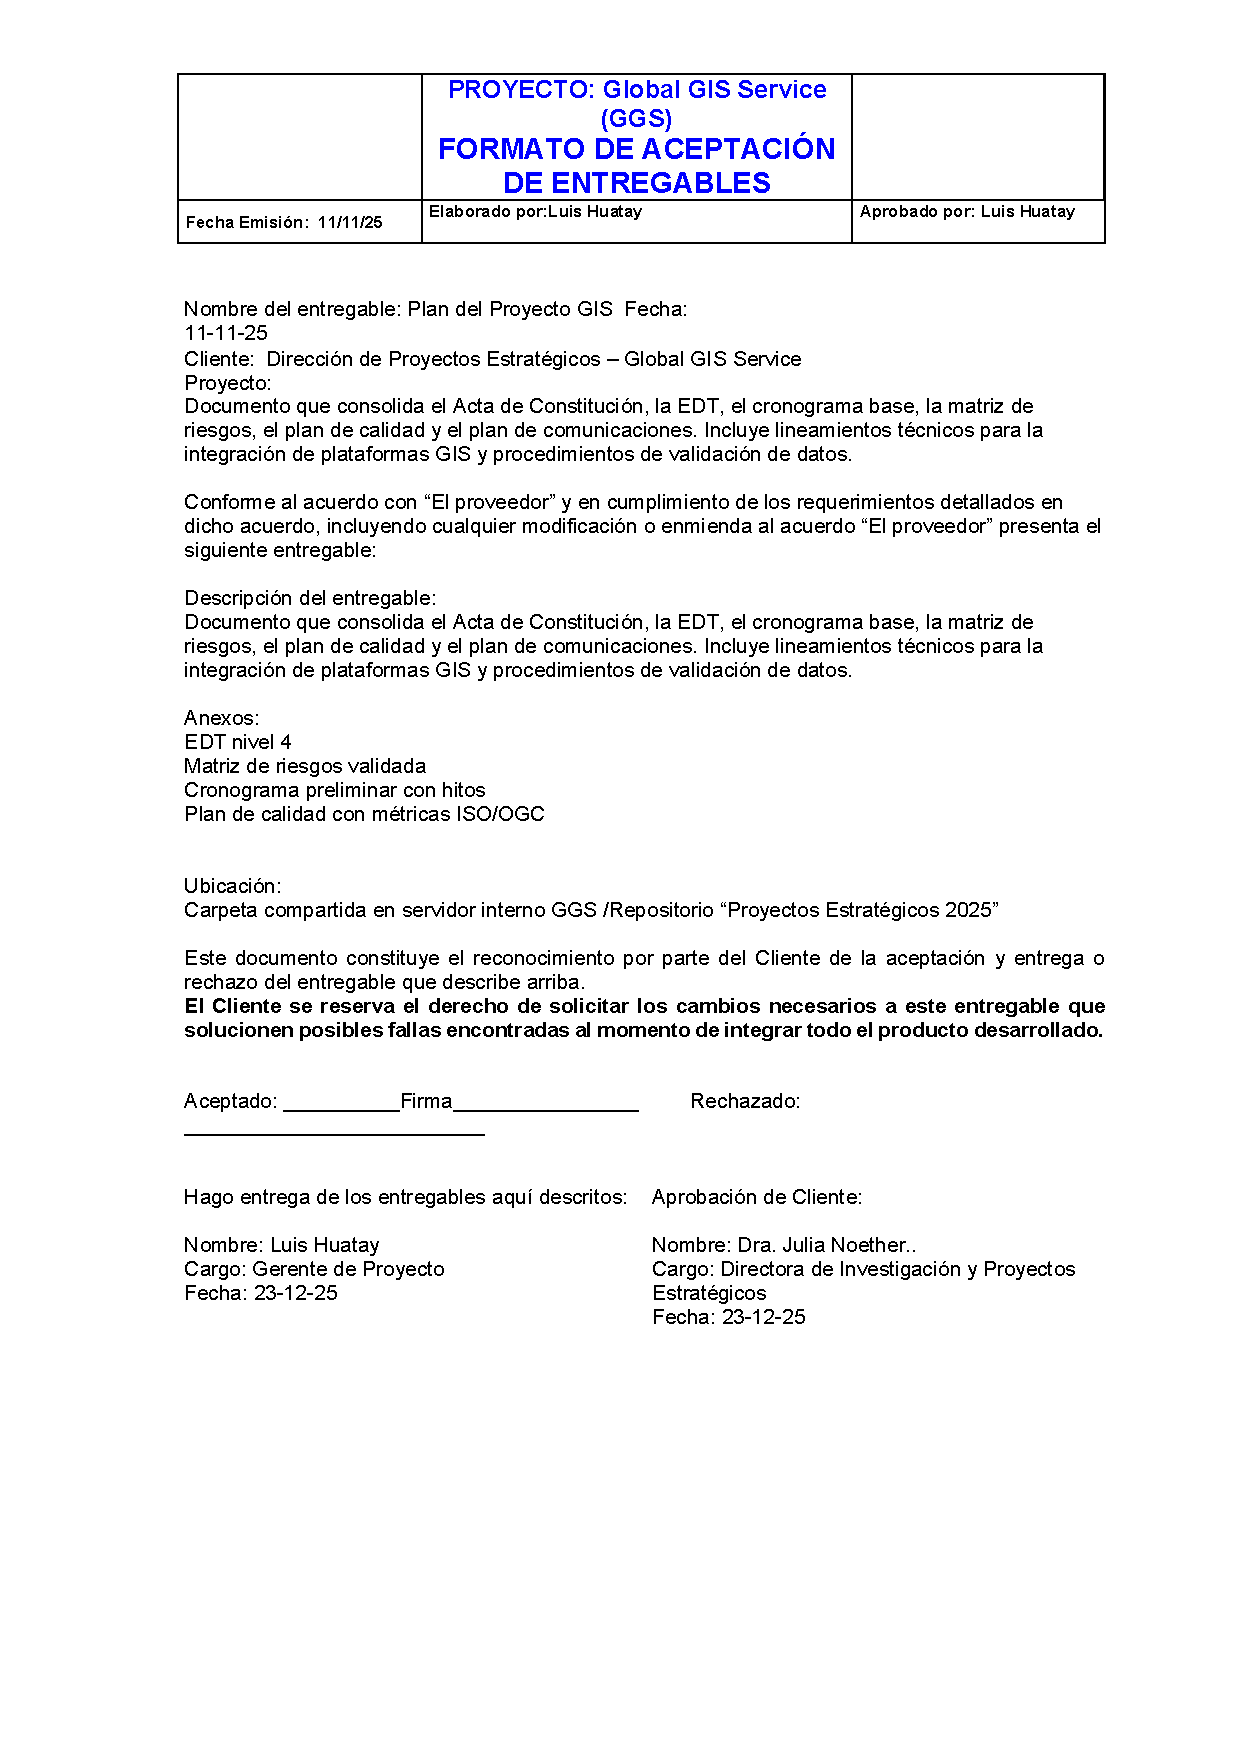
\includepdf[pages=-]{a2.pdf}

\subsection{Gestión del Cronograma}

    El seguimiento de la gestión del cronograma del proyecto implica monitorear el progreso del proyecto para asegurar que se complete a tiempo. Esto incluye la definición de las actividades, la secuenciación de las actividades, la estimación de la duración de las actividades, el desarrollo del cronograma y el control del cronograma.


    \textbf{Objetivo:} Asegurar que el proyecto se complete dentro del tiempo planificado, identificando y gestionando cualquier desviación del cronograma.

    Durante dicha fase, se utiliza el siguiente formato para reportar el avance semanal del proyecto. El seguimiento del cronograma es fundamental para identificar retrasos y tomar medidas correctivas oportunas. Eso se refleja en el siguiente reporte de avance semanal:

  El reporte de seguimiento semanal proporciona una visión detallada del progreso del proyecto, incluyendo las actividades completadas, los hitos alcanzados y cualquier desviación del plan original. Este documento sirve como herramienta fundamental para la toma de decisiones y la implementación de acciones correctivas.

  La actualización regular del cronograma permite al equipo identificar tempranamente posibles retrasos o problemas, facilitando la asignación efectiva de recursos y la adaptación del plan según sea necesario. Mediante este seguimiento sistemático, se mantiene la transparencia en la comunicación con los interesados y se asegura el cumplimiento de los plazos establecidos.

\subsection{Gestión de la calidad}

    La gestión de la calidad del proyecto implica asegurar que el proyecto cumpla con los requisitos y estándares de calidad establecidos. Esto incluye la planificación de la calidad, la gestión de la calidad y el control de la calidad.

    \textbf{Objetivo:} Asegurar que los entregables del proyecto cumplan con los estándares de calidad requeridos, satisfaciendo las expectativas de los interesados.

    A continuación se presenta un ejemplo de informe de control de calidad utilizado en el proyecto.

    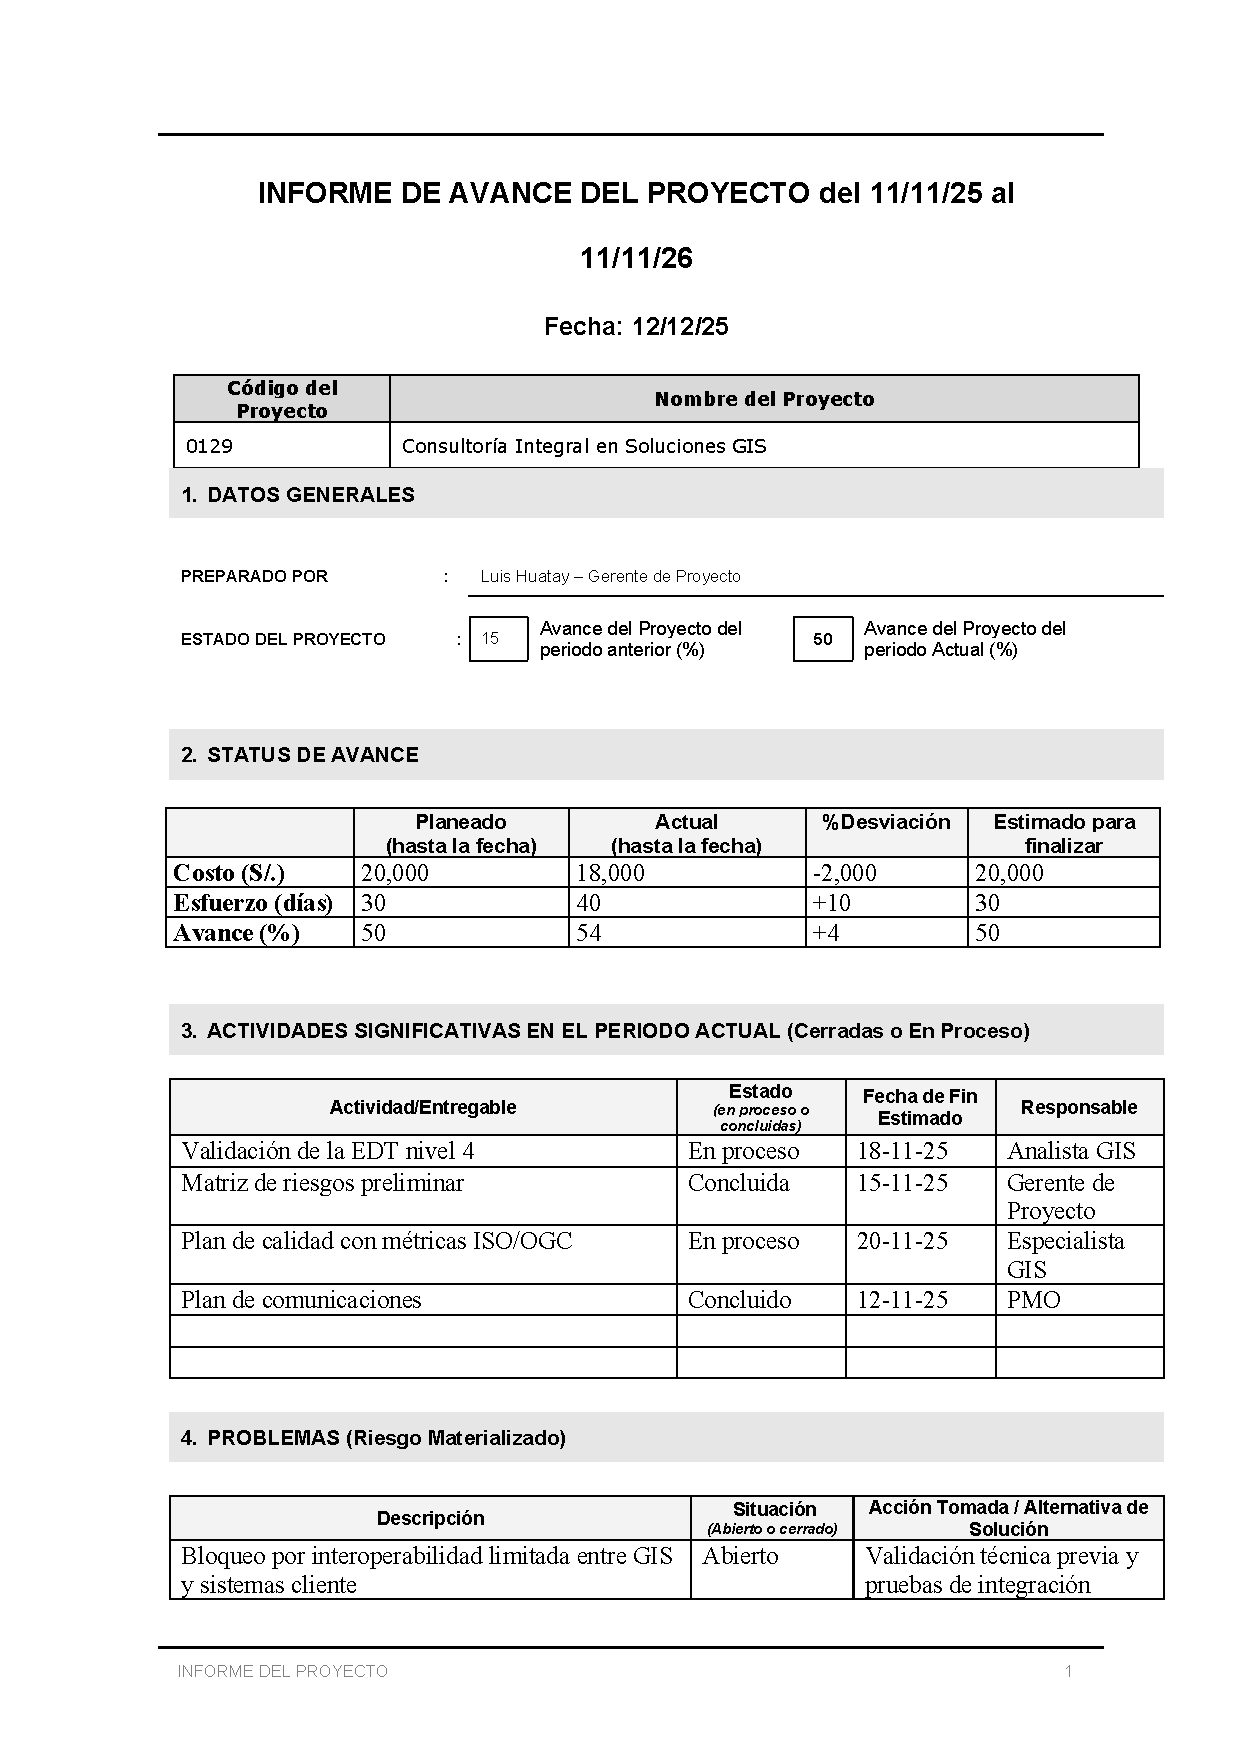
\includepdf[pages=-]{a3.pdf}

    \subsection{Gestión de los Recursos}

    La gestión de los recursos del proyecto implica planificar, adquirir, desarrollar y gestionar el equipo del proyecto. Esto incluye la planificación de los recursos, la estimación de los recursos, la adquisición de recursos, el desarrollo del equipo y la gestión del equipo.

    \textbf{Objetivo:} Asegurar que el equipo del proyecto esté bien organizado, motivado y capacitado para cumplir con los objetivos del proyecto.

    
    En lo que respecta a la gestión de recursos humanos, se ha implementado un plan de desarrollo del equipo que incluye capacitaciones y actividades de integración para mejorar la cohesión y el rendimiento del equipo. Además, se han establecido mecanismos de comunicación efectivos para asegurar que todos los miembros del equipo estén alineados con los objetivos del proyecto.

    \subsection{Gestión de las Comunicaciones}

    La gestión de las comunicaciones del proyecto implica planificar, gestionar y controlar las comunicaciones del proyecto. Esto incluye la planificación de las comunicaciones, la gestión de las comunicaciones y el control de las comunicaciones.

    \textbf{Objetivo:} Asegurar que la información del proyecto se comunique de manera efectiva a todos los interesados, facilitando la toma de decisiones y la colaboración.

    Se ha establecido un plan de comunicaciones que define los canales, frecuencia y formatos de comunicación para mantener a todos los interesados informados sobre el progreso del proyecto. Además, se han implementado reuniones regulares de seguimiento y reportes de avance para asegurar una comunicación fluida y efectiva.

    \subsection{Gestión de los Riesgos}

    La gestión de los riesgos del proyecto implica identificar, analizar y responder a los riesgos del proyecto. Esto incluye la planificación de la gestión de riesgos, la identificación de riesgos, el análisis cualitativo y cuantitativo de riesgos, la planificación de respuestas a los riesgos y el control de riesgos.

    \textbf{Objetivo:} Minimizar el impacto de los riesgos en el proyecto, asegurando que se tomen medidas proactivas para gestionar los riesgos identificados.

    Se ha desarrollado un registro de riesgos que documenta todos los riesgos identificados, sus análisis y las estrategias de mitigación implementadas. Además, se realizan revisiones periódicas del registro de riesgos para identificar nuevos riesgos y evaluar la efectividad de las respuestas a los riesgos existentes.

    \subsection{Gestión de las Adquisiciones}

    La gestión de las adquisiciones del proyecto implica planificar, ejecutar y controlar las adquisiciones del proyecto. Esto incluye la planificación de las adquisiciones, la conducción de las adquisiciones y el control de las adquisiciones.

    \textbf{Objetivo:} Asegurar que los bienes y servicios necesarios para el proyecto se adquieran de manera eficiente y efectiva, cumpliendo con los requisitos del proyecto.

    Se ha establecido un proceso de adquisiciones que incluye la selección de proveedores, la negociación de contratos y la gestión de las relaciones con los proveedores. Además, se monitorean las adquisiciones para asegurar que se cumplan los plazos, costos y calidad establecidos en los contratos.

    \subsection{Gestión de las Adquisiciones}

    La gestión de las adquisiciones del proyecto implica planificar, ejecutar y controlar las adquisiciones del proyecto. Esto incluye la planificación de las adquisiciones, la conducción de las adquisiciones y el control de las adquisiciones.

    \textbf{Objetivo:} Asegurar que los bienes y servicios necesarios para el proyecto se adquieran de manera eficiente y efectiva, cumpliendo con los requisitos del proyecto.

    Se ha establecido un proceso de adquisiciones que incluye la selección de proveedores, la negociación de contratos y la gestión de las relaciones con los proveedores. Además, se monitorean las adquisiciones para asegurar que se cumplan los plazos, costos y calidad establecidos en los contratos.

A continuación se presenta un ejemplo de contrato utilizado en el proyecto.

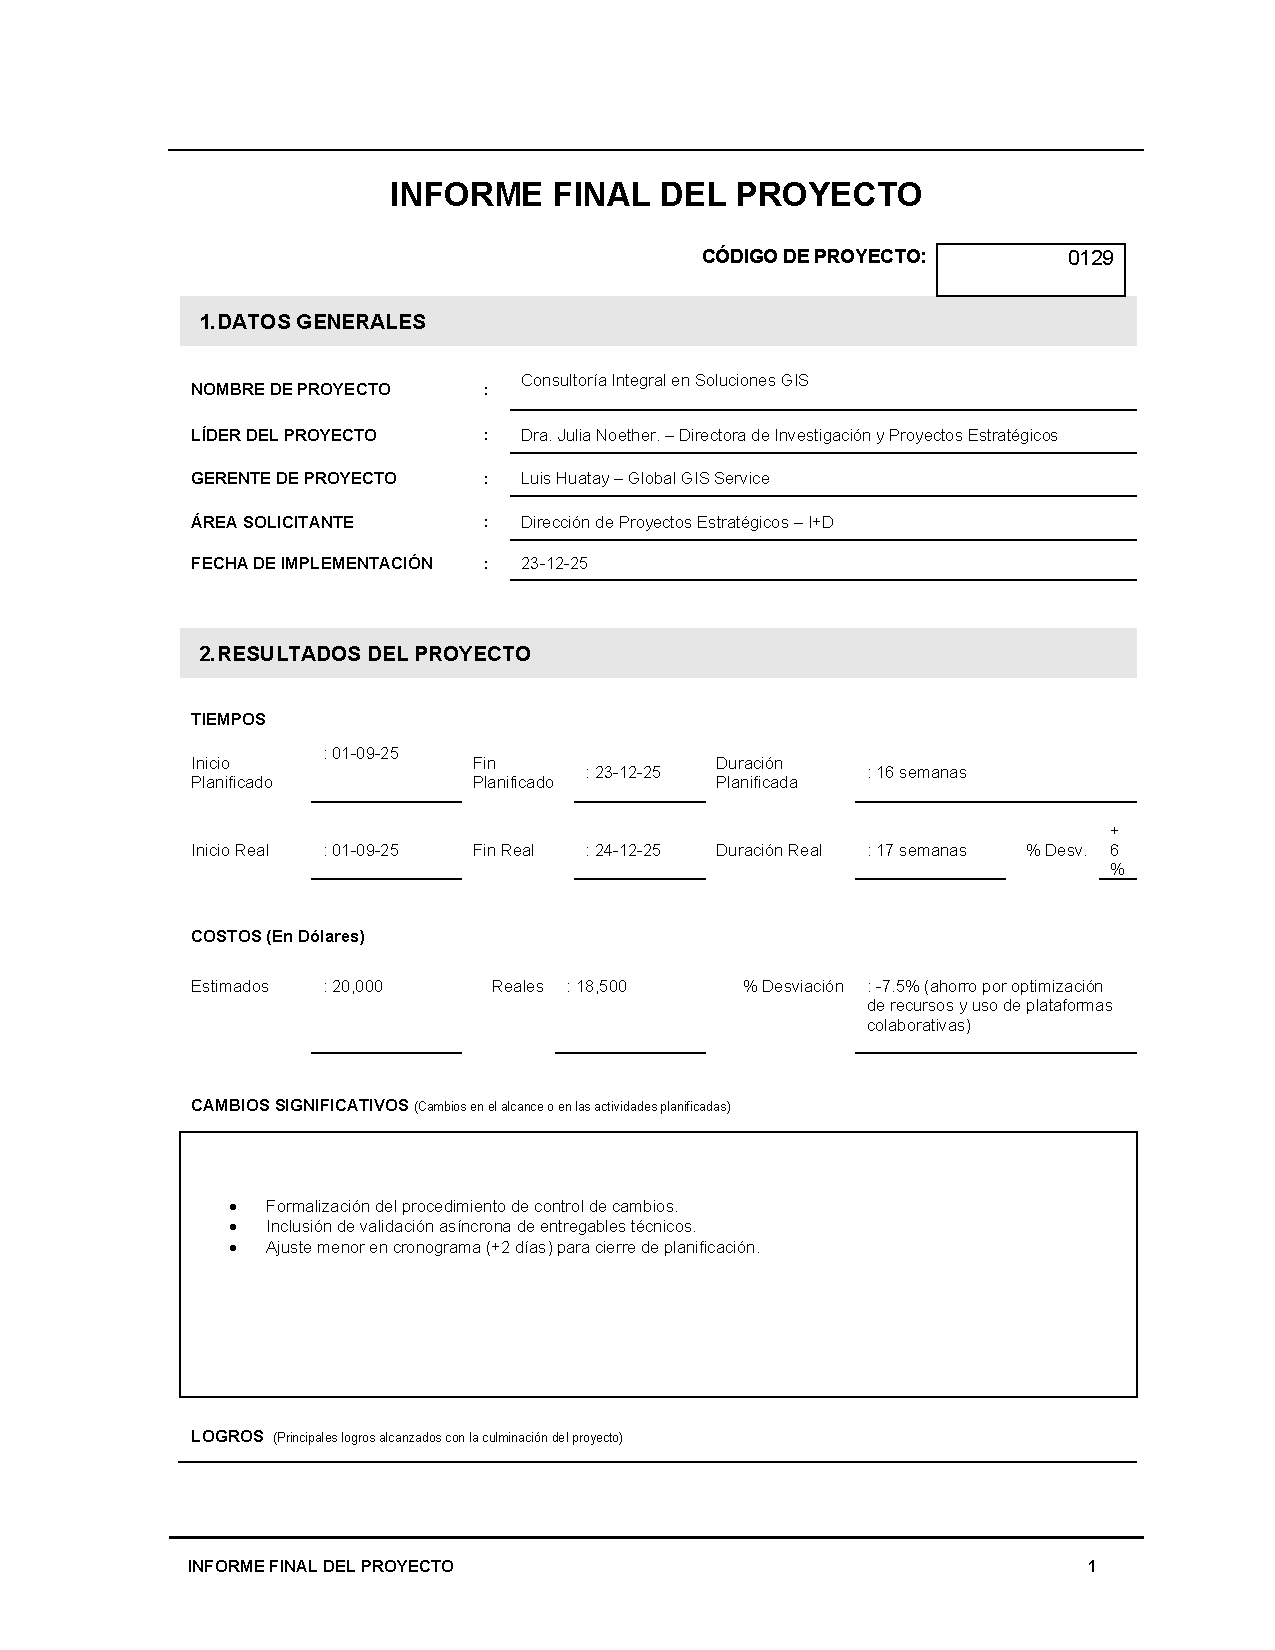
\includepdf[pages=-]{a4.pdf}

\section{Conclusiones:}

\begin{enumerate}
  \item Los procesos de seguimiento y control integrados garantizan la alineación continua entre alcance, tiempo, costo y calidad; un plan de gestión claro y un control integrado de cambios facilitan la toma de decisiones y reducen riesgos de desalineación.
  \item La gestión del alcance y del cronograma, apoyada en reportes semanales y mecanismos de verificación, permite la detección temprana de desviaciones y la aplicación oportuna de acciones correctivas para cumplir los plazos y evitar alcance no planificado.
  \item La gestión de calidad, recursos y comunicaciones —respaldada por informes, capacitación y canales definidos— incrementa la probabilidad de entregar productos conformes y mejora la coordinación y el desempeño del equipo.
  \item La gestión de riesgos y adquisiciones, con registros y contratos documentados, aporta trazabilidad y control sobre proveedores y contingencias; se recomienda mantener revisiones periódicas y actualización de registros para fomentar la mejora continua."
\end{enumerate}